% Drawing 74/02-10 -- folder 74, batch 02, archive page 38 (PDF page 39).
% Transcription: dans la marge gauche, un petit schéma : deux paires de points $x, y$ et $x', y'$ reliées par des flèches courbes en sens opposés, autour d'un axe vertical.
% Kind: two pairs of points exchanged by arrows about an axis. Method 2 (schematic redraw from the facsimile). Status: partial.
% Notes: A vertical axis. At the top two curved arrows in opposite senses: one over the axis to the right, one just under it back to the left. At the bottom one curved arrow across the axis with heads at both ends (the right one overwritten). A thin oblique stroke runs from the upper right down to the axis. The letters x, y (top) and x', y' (bottom) are placed by reading; a cross marks the lower left point. Nothing is struck. Overlay check 2026-11-13 (issue 147, Claude claude-opus-5-5): the redraw, rasterised by the skill's previewer (not compiled: no TeX in the session), laid over the 300 dpi colour crop of the scan (261 ppi). The axis began 10 units too high (on the page it starts under the upper arrow) and the arrows lay 1 to 2 units off: the axis and the three arrows are redrawn through points read on their ink, and the thin oblique stroke, which the earlier redraw lacked, is added. Still differs: between and beside the arrows the page has scrawled marks (a large looped stroke like a « 3 » across the axis under the upper arrows, a hook at the left end of the upper arrow, short ticks and two primes at the bottom) which the transcription reads as the letters x, y, x', y'; they are not legible as letters, so they are not drawn stroke by stroke and the letters stand where the transcription's reading puts them.
% Coordinates: 1 unit = 1 mm = 1/100 of the crop width (bbox in page fractions: [0.1, 0.53, 0.26, 0.67]).
% Redrawn by Claude (claude-opus-5-5), issue #73, 2026-11-09; not checked by a human; not compiled (no TeX in the session).
% Checked by Claude (claude-opus-5-5) 2026-11-13 (issue #147): overlaid on the 300 dpi colour facsimile and corrected; not compiled (no TeX in the session). Status: partial.
% Rights: reproduces part of the work -- behind RENDER_TRANSCRIPTS, never published by itself.
\documentclass[tikz,border=3pt]{standalone}
\usepackage{amsmath,amssymb}
\usetikzlibrary{patterns,arrows.meta}
\tikzset{pencil/.style={black!45}, struck/.style={black!35}, mark/.style={circle,draw,inner sep=1.3pt}, pt/.style={circle,fill,inner sep=0.9pt}, opt/.style={circle,draw,fill=white,inner sep=1.1pt}}
\begin{document}
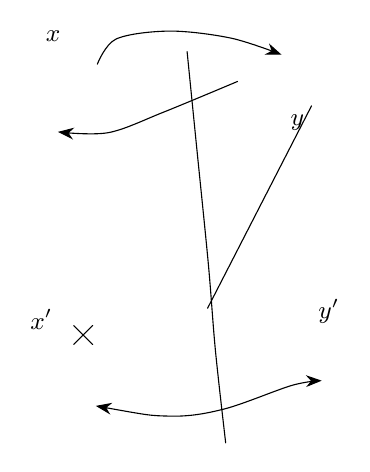
\begin{tikzpicture}[x=1mm,y=1mm,line cap=round,line join=round,font=\scriptsize]
\draw plot[smooth, tension=0.55] coordinates {(47,-28) (48.2,-40) (49.7,-55) (50.6,-66) (51.9,-77.7)};
\draw[-{Stealth[length=2mm]}] plot[smooth, tension=0.55] coordinates {(35.6,-29.6) (38,-26.4) (44.8,-25.4) (52.6,-26.3) (59,-28.4)};
\draw[-{Stealth[length=2mm]}] plot[smooth, tension=0.55] coordinates {(53.4,-31.8) (44,-35.7) (37,-38.3) (30.6,-38.2)};
\draw[{Stealth[length=2mm]}-{Stealth[length=2mm]}] plot[smooth, tension=0.55] coordinates {(35.4,-73) (44.8,-74.3) (51.7,-73.4) (60.3,-70.4) (64.1,-69.8)};
\draw (62.8,-34.9) -- (49.6,-60.6);
\node[inner sep=1pt] at (30,-26) {\small $x$};
\node[inner sep=1pt] at (61,-37) {\small $y$};
\node[inner sep=1pt] at (28.5,-62) {\small $x'$};
\node[inner sep=1pt] at (65,-61) {\small $y'$};
\draw (32.6,-62.8) -- (35,-65.2);
\draw (32.6,-65.2) -- (35,-62.8);
\end{tikzpicture}
\end{document}
